\documentclass[a4paper]{article}

\usepackage[english]{babel}
\usepackage[utf8]{inputenc}
\usepackage{amsmath}
\usepackage{graphicx}
\usepackage[colorinlistoftodos]{todonotes}
\usepackage{hyperref}

\title{Capstone Project for Udacity Machine Learning Nanodegree}

\author{Pär Steffansson}

\date{\today}

\begin{document}
\maketitle

\tableofcontents

\section{Project Definition}
An overview of the project definition is described below. For more details see the competition
\href{https://www.kaggle.com/c/zillow-prize-1#description}{Zillow Prize}.

\subsection{Project Overview}
%
% Student provides a high-level overview of the project in layman’s terms. Background information such as the
% problem domain, the project origin, and related data sets or input data is given.
%
I selected the competition \href{https://www.kaggle.com/c/zillow-prize-1#description}{Zillow Prize} found at \href{https://www.kaggle.com}{Kaggle} as the Capstone project in my \textit{Machine Learning Engineer Nanodegree} provided by \href{https://www.udacity.com}{Udacity}.

\href{https://www.zillow.com}{Zillow} is the leading real estate and rental marketplace dedicated to empowering consumers with data. They launched the Kaggle competition \textit{Zillow Prize} to improve their ability to predict house prices.

I selected this competition to learn from the rich source of knowledge the community around these competitions provide. Comparing and learning from public Kernels provided gives a good benchmark of cutting edge models for these kind of problems.

\subsection{Problem Statement}
%
% The problem which needs to be solved is clearly defined. A strategy for solving the problem,
% including discussion of the expected solution, has been made.
%
They have been developing their own model to predict prices for years. The problem at hand is to see if the Kaggle community can improve on it creating an even better model. 

Zillow provide an error from using their own model trying to predict estate prices. The problem is to predict that error. This is a regression task and a weighted solution of three models will be used. First model is a simple model where the mean of the training data is the prediction for all estates. Second and third model are two different tree based Gradient boosting models called LightGBM and XGBoost.

\subsection{Metrics}
%
% Metrics used to measure performance of a model or result are clearly defined. Metrics are 
% justified based on the characteristics of the problem.
%
Zillow is asking to predict the \textit{logerror} between their Zestimate model and the
actual sale price, given all the features of a home. The \textit{logerror} is defined as
\[ logerror = log(Zestimate) - log(SalePrice) \]
\textit{Mean Absolute Error} (MAE) is then used as the metric on the logerror individually for Mean, LightGBM, XGBoost, and Weighted model. It's simple and fast to compute and works well with selected models. The formula is 
\[ MAE(y_{true}, y_{pred}) = \frac{1}{n} \sum_{i=1}^{n} |y_{pred}(i) - y_{true}(i)| \]


\section{Analysis}

\subsection{Data Exploration}
% If a dataset is present, features and calculated statistics relevant to the problem have 
% been reported and discussed, along with a sampling of the data. In lieu of a dataset, 
% a thorough description of the input space or input data has been made. Abnormalities or
% characteristics about the data or input that need to be addressed have been identified.
% Exploratory Visualization
% A visualization has been provided that summarizes or extracts a relevant characteristic 
% or feature about the dataset or input data with thorough discussion. Visual cues are 
% clearly defined.
This data exploration is inspired by the \href{https://www.kaggle.com/sudalairajkumar/simple-exploration-notebook-zillow-prize}{Simple Exploration Notebook - Zillow Prize} written by Kaggle Grandmaster \href{https://www.kaggle.com/sudalairajkumar}{SRK}.

We will be working with following data files
\begin{itemize}
    \item \textit{properties\_2016.csv} contains all the properties with their home features for 2016. Note: Some 2017 new
    properties don't have any data yet except for their parcelid's. Those data points should be populated when
    properties\_2017.csv is available.
    \item \textit{train\_2016.csv} contains the training set with transactions from 1/1/2016 to 12/31/2016.
    \item \textit{sample\_submission.csv} is a sample submission file in the correct format
\end{itemize}

\subsubsection{Training Set File}
The training set in file \textit{train\_2016.csv} contains 90275 rows and three columns
\begin{itemize}
    \item \textit{parcelid} is the id of the property.
    \item \textit{logerror} is the log of the error comparing the log of the actual price and the log of the predicted price.
    \item \textit{transactiondate} is the date when the property was sold
\end{itemize}

Each row correspond to a property transaction and there will be more than one row in this file with the same parcelid if the property has been sold more than ones during 2016. In fact counting there are
\begin{itemize}
    \item 90026 properties that have been sold ones
    \item 123 properties that have been sold twice
    \item and one property that was sold three times.
\end{itemize}

\begin{figure}
\centering
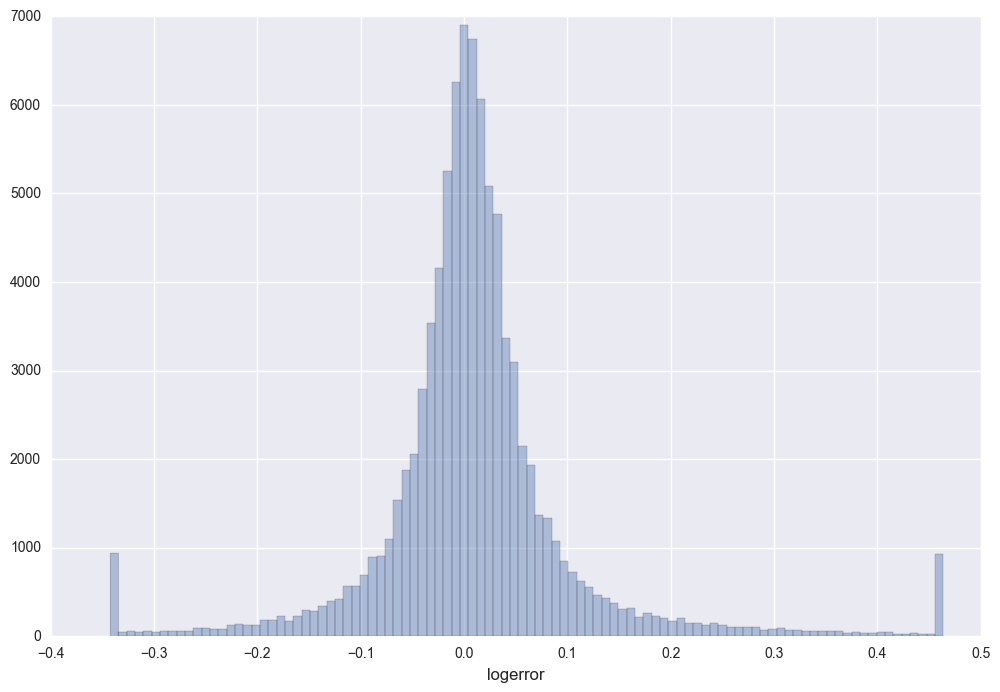
\includegraphics[width=1\textwidth]{./img/train-logerror.png}
\caption{\label{fig:logerror}Logerror distribution}
\end{figure}
Looking at Figure \ref{fig:logerror} the logerror has a nice normal distribution centered around zero.

\begin{figure}
\centering
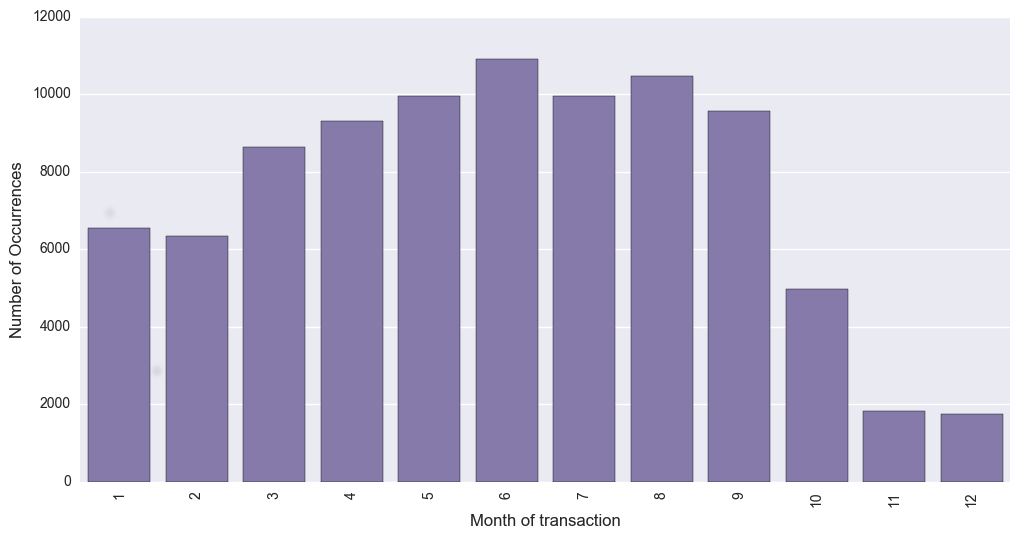
\includegraphics[width=1\textwidth]{./img/train-transactiondate.png}
\caption{\label{fig:transactions}Number of transactions over time}
\end{figure}
According to Zillow the training data has all the transactions before October 15, 2016, plus some of the transactions after October 15, 2016. Looking at Figure \ref{fig:transactions} from January to September there are about 6000-11000 transactions per month while dropping to under 2000 in November to December.

\subsubsection{Properties}
Property data file \textit{properties\_2016.csv} is a lot larger with 2985217 rows and 58 columns describing home features. It seems like some of the columns contain less information in the form of NaN values.
\begin{figure}
\centering
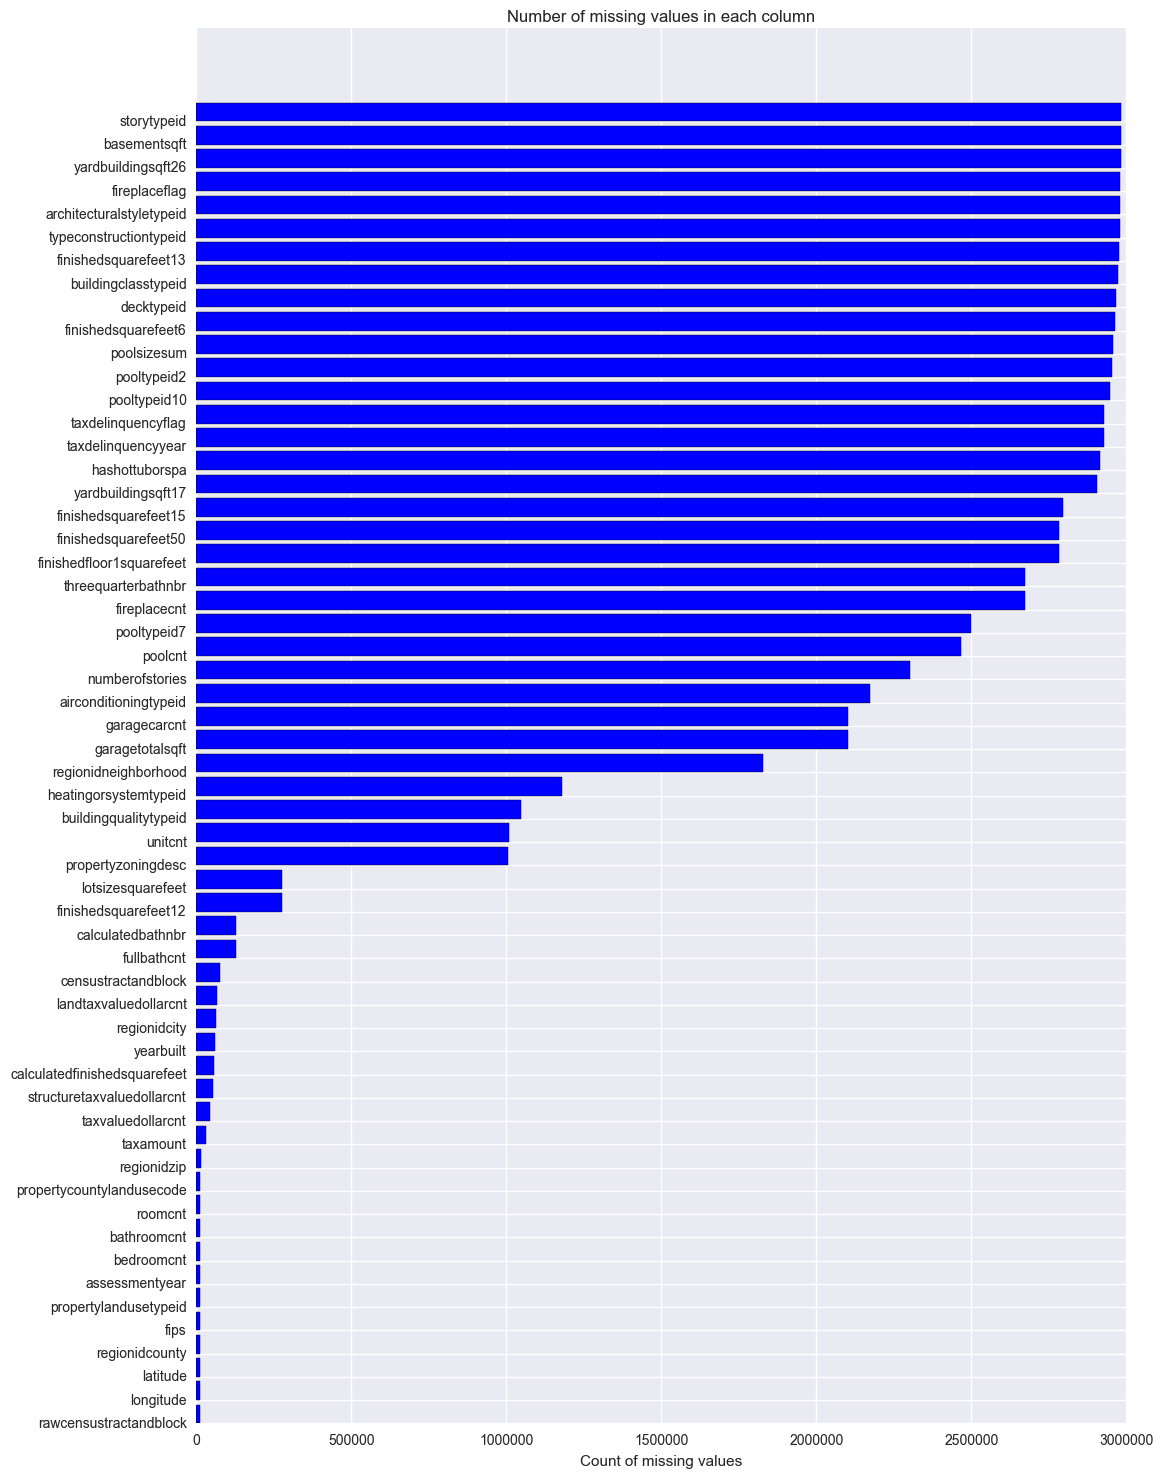
\includegraphics[width=1\textwidth]{./img/prop-nan.png}
\caption{\label{fig:prop-nan} Amount of information in features}
\end{figure}
Looking at Figure \ref{fig:prop-nan} more than half of the data is not there and the data loss is unevenly distributed on features. About 30 percent of the features will most likely not contribute to a better model when they do not contain any information.

\begin{figure}
\centering
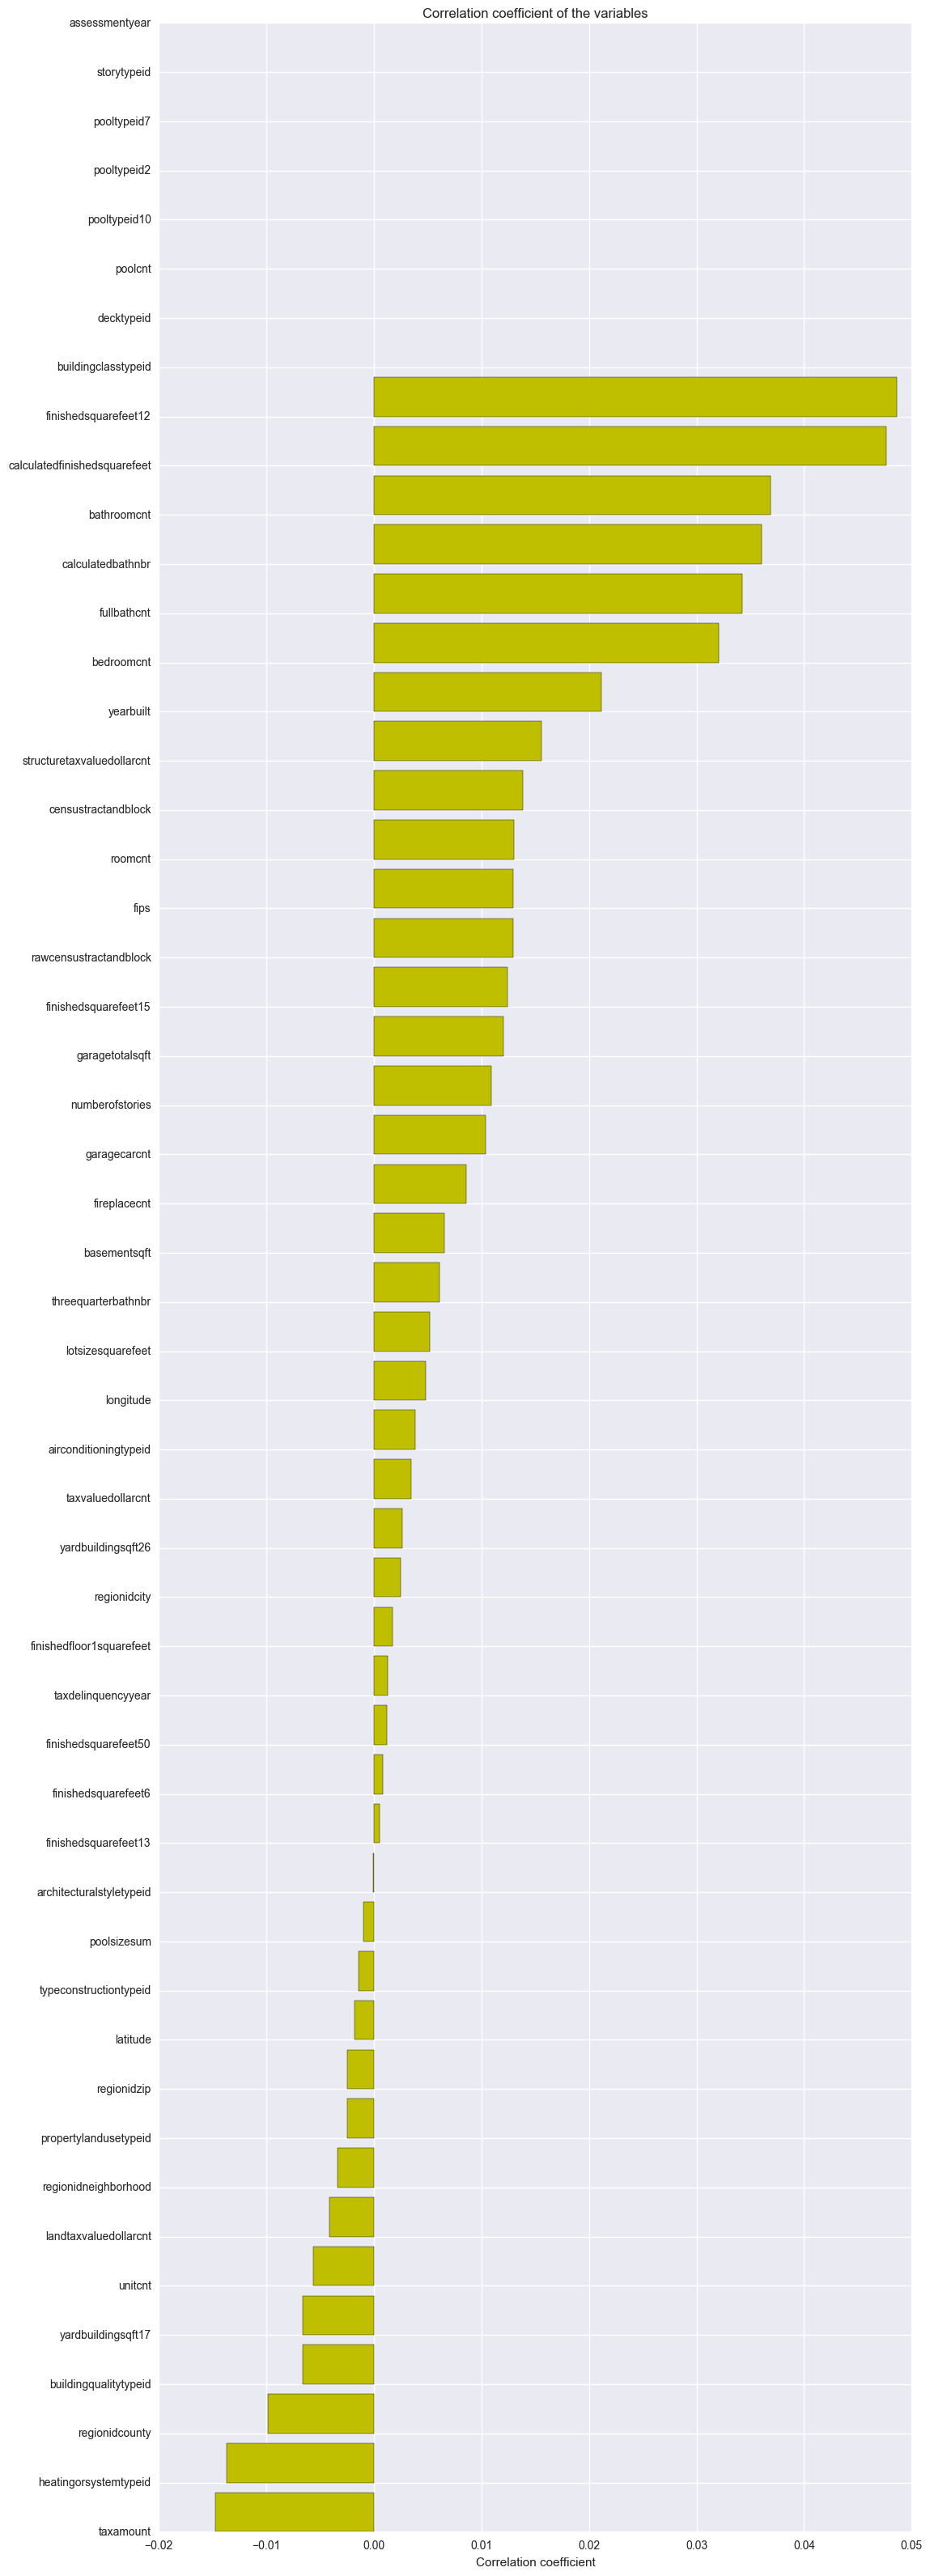
\includegraphics[width=0.6\textwidth]{./img/prop-important.png}
\caption{\label{fig:prop-important} Correlation between features and the log error}
\end{figure}
There are many features, so let take a look at the correlation between the logerror and these features to see which ones seems to be more likely to improve the prediction than others. Looking at Figure \ref{fig:prop-important} we can see
\begin{itemize}
    \item correlation is low in general which indicate that improving prediction will be hard
    \item a few features are missing correlation most likely because there are only one value
\end{itemize}

\begin{figure}
\centering
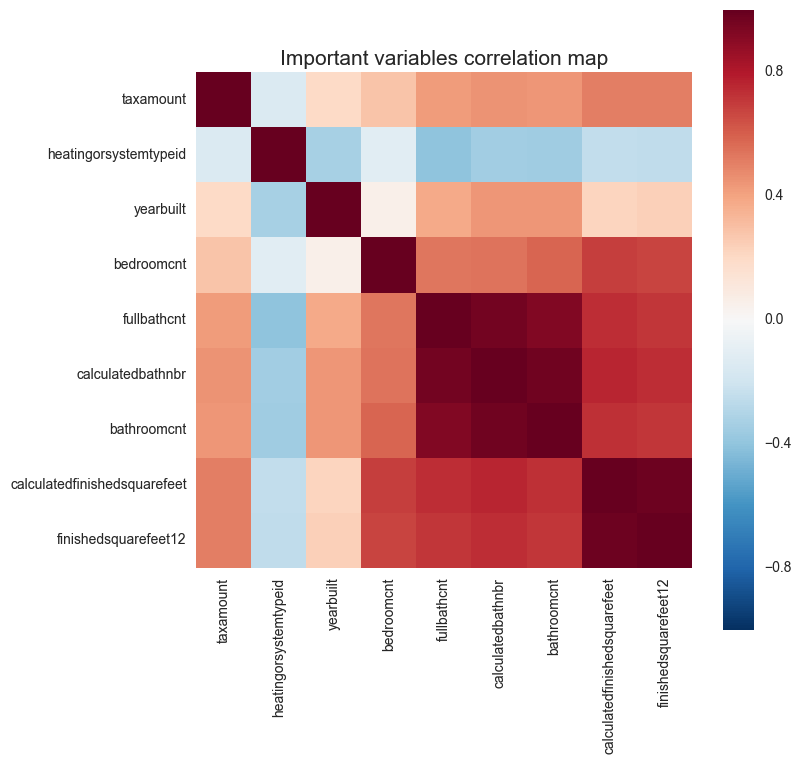
\includegraphics[width=1\textwidth]{./img/prop-corr-feature.png}
\caption{\label{fig:prop-corr-feature} Correlation between features and the log error}
\end{figure}
If we look at features with a correlation less than -0.01 and more than 0.02 we may filter out nine features. High correlation between these features might indicate that they contain the same type of information which most likely makes prediction harder than if little correlation exists. Looking at Figure \ref{fig:prop-corr-feature} show quite high correlation between features, especially between features relating to room counts and house size.

% TODO: add no pattern for major features


\subsection{Algorithms and Techniques}
% Algorithms and techniques used in the project are thoroughly discussed and properly 
% justified based on the characteristics of the problem.
\subsubsection{Overview}
I have selected the approach of weighing the result of following three different algorithm.
\begin{itemize}
    \item
        \textit{Mean} which is the simple prediction of predicting all by the mean of the training data. The logerror seems to follow the normal distribution and this is the mean that we are after and is estimated by the mean of the training data.
    \item
        \textit{LightGBM} is a gradient boosting framework that uses tree based learning algorithms. It is a high speed, high accuracy, and large scale data library.
    \item
        \textit{XGBoost} implements the gradient boosting tree based model as well. The library is optimized to be a scalable, portable and accurate library.
\end{itemize}
LightGBM and XGBoost are tree based Gradient boosting models. The result from these three models will then be weighted according to the best weights found using the training set. Often the result of weighing the result from different models creates a better result then any of the models by them self

\subsubsection{Gradient Tree Boosting Models}
Gradient tree boosting can be used for regression and classification which produce prediction by ensemble of weak decision trees.

A decision tree predicts a label by starting at the root of the tree, selecting branches at every node using the feature base statement defined at each node, ending up in a leaf which contains the prediction. A weak decision tree is a tree that have few leaves (generally 4-8 leafs).

In Gradient boosting weak decision trees are added one at a time. Once a tree is added, it will not change. A new tree is added such that the loss is reduced. This is done by parameterize the tree and changing the parameters using the gradient decent.

Gradient boosting tree has excellent accuracy which is the main reason for using it in this problem. Correlation between the logerror and features are low which indicate that a sensitive algorithm is needed to be able to predict the logerror. However, Gradient boosting trees are prone to overfit so extra caution must be taken tuning parameters.

In general, Gradient tree boosting models has proven to produce good predictions.

\subsection{Benchmark}
% Student clearly defines a benchmark result or threshold for comparing performances of solutions obtained.
The closer to zero the \textit{Mean Absolute Error} metric is, the better the model performance. The model result will also be compared with the \textit{Zero model} which is the simple model of predicting the logerror to always be zero independent of feature values. The error metric of the Zero model is used as an upper level when comparing. The Zero model will product a MAE logerror value of 0.053989.


\section{Methodology}

\subsection{Data Preprocessing}
% All preprocessing steps have been clearly documented. Abnormalities or characteristics 
% about the data or input that needed to be addressed have been corrected. If no data 
% preprocessing is necessary, it has been clearly justified.
The data is prepared in following steps before fed to LightGBM and XGBoost.
\begin{enumerate}
    \item Remove outliers to prevent the model to reduce generalization due to data points not likely to reflect possible future data. Outliers was defined as before the first and after the 99 percentile.
    \item Convert types so that the data can be used in LightGBM and XGBoost
    \item Enriching the train data in file \textit{train\_2016.csv} with property data in file
        \textit{properties\_2016.csv} by joining on \textit{parcelid}
    \item Adding the month of the transaction as a feature
    \item Removed columns \textit{parcelid} and \textit{transactiondate} since these will most likely not improve the prediction
    \item Split data into train and test
\end{enumerate}

\subsection{Implementation}
% The process for which metrics, algorithms, and techniques were implemented with the 
% given datasets or input data has been thoroughly documented. Complications that 
% occurred during the coding process are discussed.
\subsubsection{Libraries}
Numpy is used to handle all statistical ground work, like removing outliers, converting data types, and mean computations. Scikit-learn was used to compute MAE and split data into a train and test set. Panda was used to read and write data to disk and merge data sets. LightGBM and XGBoost are two libraries that need to be downloaded and installed separately. 


\subsubsection{Overview}
The implementation is divided up into two parts, training and the test part. The data is also divided into two parts. The test size of the data is 33\% while the train size is 67\%. A random state seed was used everywhere to enable identical runs.

The Mean, LightGBM, and XGBoost is first trained individually. Parameters for LightGBM and XGBoost are tuned independent of each other. Once all three models are trained and tuned, the weights are trained by randomly select the weights over and over again until a minimum MAE is obtained on the weighted sum. To prevent overfitting the weights, a minimum weight of 0.1 is set for LightGBM and XGBoost. 


\subsubsection{Pseudocode}

The overall implementation steps are
\begin{enumerate}
    \item Preprocessing and train for LightGBM using train data
    \item Preprocessing and train for XGBoost using train data
    \item Find the best weights for the tree models by randomly trying different values on the train result from above. I selected a minimum weight of 0.1 for the LightGBM and XGBoost models.
    \item Predict \textit{logerror} for test data using LightGBM
    \item Predict \textit{logerror} for test data using XGBoost
    \item Predict final \textit{logerror} for test data weighing together LightGBM, XGBoost, and the constant model using the weights from above.
    \item Compute the performance using the Mean Absolute Error metric
    \item Adjust configuration parameters for LightGBM and XGBoost and start over at the top
\end{enumerate}


\subsubsection{Complications}
Preparing the data so that LightGBM and XGBoost would not crash took a lot of time. Data type transformations were needed.

The sum of the weights for the three models need to be 1.0 while each weight is positive. At first I did not check for positive weights and this generated a less accurate Weighted model. 

Before adding the lower limit on the weights of 0.1 for LightGBM and XGBoost the XGBoost got most of the weights which generated a worse test. The lower limit contributed to allowing the Weighted model to generalize better.


\subsection{Refinement}
% The process of improving upon the algorithms and techniques used is clearly documented. Both the initial and
% final solutions are reported, along with intermediate solutions, if necessary.
Major parameters for both models where tuned through the steps of changing one parameter at a time to different values while rerunning the prediction and see if the train and test data result improved. In case of
\begin{enumerate}
    \item neither train result nor test result improved indicates that the change made made the model worse and the change was reverted
    \item train result improved but the test result become worse indicates that the change made made the model overfit and the change was reverted
    \item train result and the test result improved indicates that the change made the model generalize better and the change was kept
\end{enumerate}

Following improvements were made per model.
\subsubsection{LightGBM}
\begin{itemize}
    \item Changed learning rate from default value of 0.1 to 0.0021 which mitigated overfitting
    \item Changed number of leaves in one tree from default value of 31 to 512 which improved result
\end{itemize}
\subsubsection{XGBoost}
\begin{itemize}
    \item Changed the step size shrinkage (eta) from default value of 0.3 to 0.03295 which mitigated overfitting
    \item Changed the maximum depth of a tree from default value of 6 to 8 which improved the model without overfitting it by increasing complexity
    \item Changed the subsample ratio from default value of 1 to 0.8 which mitigated overfitting
\end{itemize}


\section{Results}

\subsection{Mean Absolute Errors}
Mean Absolute Error and Weights for the \textbf{training} data was
\begin{center}
\begin{tabular}{ l l l }
    \textbf{Model} & \textbf{Error} & \textbf{Weights} \\
    Mean & 0.053027 & 0.002130 \\
    LightGBM & 0.049524 & 0.104294 \\
    XGBoost  & 0.048911 & 0.893574 \\
    Weighted & 0.048946 & \\
\end{tabular}
\end{center}

Mean Absolute Error and Weights for the \textbf{test} data was
\begin{center}
\begin{tabular}{ l l }
    \textbf{Model} & \textbf{Error} \\
    Mean & 0.053806  \\
    LightGBM & 0.053157  \\
    XGBoost  & 0.053021  \\
    Weighted & 0.052987  \\
\end{tabular}
\end{center}


\subsection{Model Evaluation, Validation, and Justification}
% The final models qualities such as parameters are evaluated in detail. Some type of 
% analysis is used to validate the robustness of the models solution.

% The final results are compared to the benchmark result or threshold with some type 
% of statistical analysis. Justification is made as to whether the final model and 
% solution is significant enough to have adequately solved the problem.

Parameters been tuned individually and care been taken to not overfit looking at the Mean Absolute Error for training as well test data.

Changing the \textit{random state seed} will pick a different train set, pick a different test set, and train models using different entropy. Following are the seeds and errors from the different models.
\begin{center}
\begin{tabular}{ l l l l l l l }
    \textbf{Seed} & \textbf{Zero} & \textbf{Mean} & \textbf{LightGBM} & \textbf{XGBoost} & \textbf{Weighted} & \textbf{Diff} \\
    42 & 0.053989 & 0.053806 & 0.052987 & 0.053157 & 0.053021 & 0.000968 \\
    43 & 0.053258 & 0.053010 & 0.052441 & 0.052355 & 0.052313 & 0.000945 \\
    44 & 0.052686 & 0.052544 & 0.051925 & 0.051949 & 0.051889 & 0.000797 \\
    45 & 0.053565 & 0.053414 & 0.052846 & 0.052689 & 0.052660 & 0.000905 \\
\end{tabular}
\end{center}
The \textit{Diff} column is the difference between Zero model and the Weighted model and it seems to stay steady above \textbf{0.000797}. This indicates that the Weighted model can find and use some information in the data to make a better prediction than just a simple zero approach. That said, it is still a long way down to zero which means that there a lot of room for improvement.

\section{Conclusion}
Zestimate algorithm used by Zillow is doing a good job. The correlation between the logerror and
different features are low (Figure \ref{fig:prop-corr-feature}) and even if the Weighted model is utilizing some of the little information that exists to improve the result towards zero, it is not with much. It could be possible to tune the Weighted model some more but I think that it would not give much result. To make major improvements, new information is needed.

Interesting observation is that the weighing the predictions the Mean, LightGBM, and XGBoost generates a better overall MAE then for any individual model.


%\subsection{Free-Form Visualization}
% A visualization has been provided that emphasizes an important quality about the project with thorough discussion.
% Visual cues are clearly defined.

%\subsection{Reflection}
% Student adequately summarizes the end-to-end problem solution and discusses one or two particular aspects of
% the project they found interesting or difficult.

\subsection{Improvement}
% Discussion is made as to how one aspect of the implementation could be improved. Potential solutions resulting
% from these improvements are considered and compared / contrasted to the current solution.
Adding more models could improve the result, but most likely not with much. Continue tuning parameters might improve the result some more, but most likely not with much.

Adding more information is probably a better approach Using the transaction date to extract the day of the week would add information that is currently hidden. Longitude and latitude could also be used to compute distances to attractive locations like the sea or bigger cities.


\end{document}